\chapter{Zertifikate}
\section{CA}
Certificate Authorities stellen eine zentrale Stelle zum Ausgeben von Zertifkaten da. Die bekannteste dieser CA's ist Let's Encrypt~\ref{fig:lets-encrypt}, die durch das kostenlose und komplett automatisierte Austellen der Zertifikate auf viel Aufmerksamkeit von Entwicklern und Administratoren getroffen ist. 
\begin{figure}[!htb]
  \center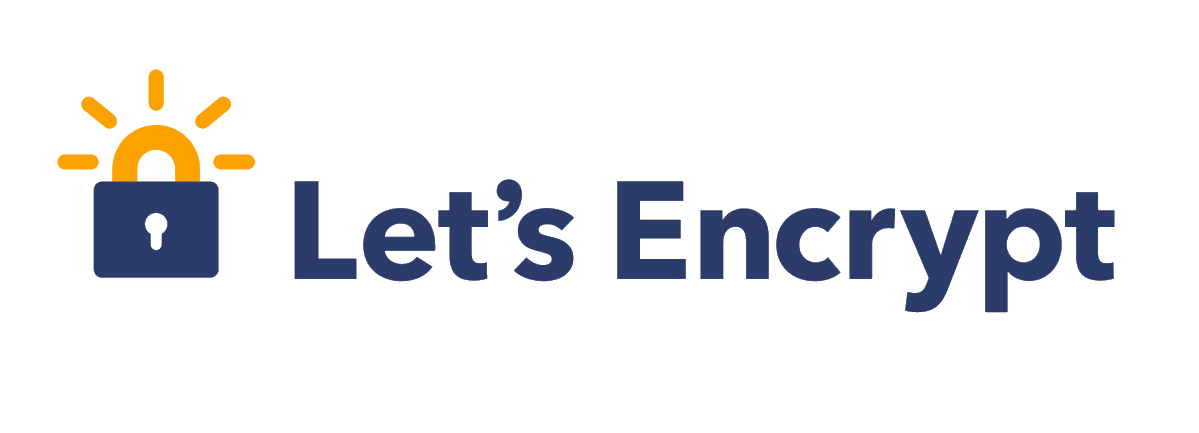
\includegraphics[scale=0.4]{images/lets-encrypt-transparent.png}
  \label{fig:lets-encrypt}
  \caption{Lets Encrypt}
\end{figure}

\section{CSR}
Um von einer CA ein Zertifkat zu bekommen, führt man einen sogenannten Certificate Signing Request durch. Dieser enthält Daten zur Identifiezierung des Antragstellenden, bspw. den FQDN\footnote{Fully Qualified Domain Name (git.kloud.software)} oder den Namen der Organisation. Der Anfragende erzeugt ein Schlüsselpaar und fügt den öffentlichen Schlüssel an den CSR an. Mit dem privaten Schlüssel wird der CSR signiert. Die CA prüft nun, ob die Signatur stimmt und die gelieferten Daten das ordnungsgemäße Ausstellen eines Zertifikates gemäß der Richtlinien der CA ermöglichen. Wenn alle Angaben valide sind, antwortert die CA mit einem Zertifikat welches mit ihrem privaten key signiert wurde.

\section{CRL}
In Certificate Revocation Lists werden Zertifikate aufgelistet, die von der CA vor dem Abauf ihrer Gültigkeit invalidiert wurden. Diese Invalidierung kann auf zwei Ebenen erfolgen. Einerseits kann ein Zertifkat den Status ``Hold'' zugewiesen bekommen, welches einer temporären Invaliderung entspricht, andererseits gibt es den Status ``Revoked'' welcher eine endgültige Invalidierung ausdrückt. Die Gründe dafür, dass ein Zertifkat auf einer CRL landet sind vielfältig:
\begin{itemize}
  \item unspecified (0)
  \item keyCompromise (1)
  \item CACompromise (2)
  \item affiliationChanged (3)
  \item superseded (4)
  \item cessationOfOperation (5)
  \item certificateHold (6)
  \item removeFromCRL (8)
  \item privilegeWithdrawn (9)
  \item AACompromise (10)
\end{itemize}
Wichtig zu beachten ist, dass das Konzept von CRL's nicht das Ablaufdatum der Zertifkate ersetzt. Ist ein Zertifkat abgelaufen, ist es immer als invalid zu betrachten. CRLs stellen jediglich ein weiteres Sicherheitsmerkmal von PKI da.
